\section{SimSite3D::Bounding\-Volume Class Reference}
\label{classSimSite3D_1_1BoundingVolume}\index{SimSite3D::BoundingVolume@{SimSite3D::BoundingVolume}}
Simple base class to define a common interface to 3D bounding volumes.  


{\tt \#include $<$Bounding\-Volume.H$>$}

Inheritance diagram for SimSite3D::Bounding\-Volume::\begin{figure}[H]
\begin{center}
\leavevmode
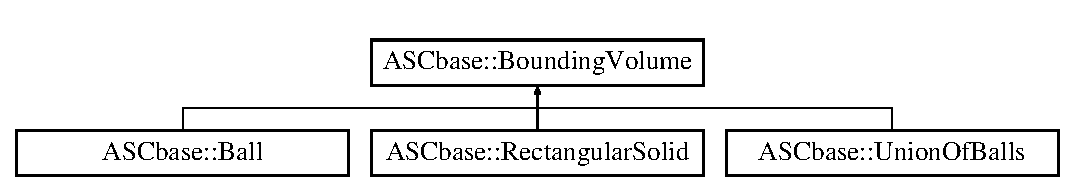
\includegraphics[height=2cm]{classSimSite3D_1_1BoundingVolume}
\end{center}
\end{figure}
\subsection*{Public Types}
\begin{CompactItemize}
\item 
\textbf{NULL\_\-VOLUME\_\-TYPE}\label{classSimSite3D_1_1BoundingVolume_90dd526306d995889c2ba0527d0e400c206c9d67d4ddcabdc42058538e90f223}

\item 
\textbf{RECTANGULAR\_\-SOLID}\label{classSimSite3D_1_1BoundingVolume_90dd526306d995889c2ba0527d0e400c978442c972efd3f68accee6a0a9f172c}

\item 
\textbf{SPHERE}\label{classSimSite3D_1_1BoundingVolume_90dd526306d995889c2ba0527d0e400cc10cb5a6a2c07cc74764081b2c34829d}

\item 
enum \textbf{volume\_\-t} \{ \textbf{NULL\_\-VOLUME\_\-TYPE}, 
\textbf{RECTANGULAR\_\-SOLID}, 
\textbf{SPHERE}
 \}
\end{CompactItemize}
\subsection*{Public Member Functions}
\begin{CompactItemize}
\item 
\bf{Bounding\-Volume} ()\label{classSimSite3D_1_1BoundingVolume_9fe70d0dcf235dd947304b1259e5dab3}

\begin{CompactList}\small\item\em Initialize pointers to NULL. \item\end{CompactList}\item 
\bf{Bounding\-Volume} (const \bf{Bounding\-Volume} \&src)\label{classSimSite3D_1_1BoundingVolume_460f07f7011383ee3bde18324fb216d8}

\begin{CompactList}\small\item\em Basic copy cstr. \item\end{CompactList}\item 
void \textbf{remove\_\-nonsurface\_\-points} (chain\_\-const\_\-iter \_\-begin, chain\_\-const\_\-iter \_\-end)\label{classSimSite3D_1_1BoundingVolume_7a552d8708eddcb0eb4b8af247eed3f3}

\item 
my\_\-float\_\-t \bf{dist\_\-to\_\-nearest\_\-grid\_\-pt} (const my\_\-float\_\-t $\ast$given\_\-pt, const my\_\-float\_\-t tol)\label{classSimSite3D_1_1BoundingVolume_29b827ac0631889832a23a6c3ccd73ad}

\begin{CompactList}\small\item\em Check if any grid point is within tolerance of given point. \item\end{CompactList}\item 
virtual bool \bf{contains} (const my\_\-float\_\-t $\ast$point) const =0\label{classSimSite3D_1_1BoundingVolume_4845f90aaeb0bdda5a7bab8ad69f249a}

\begin{CompactList}\small\item\em Is the given point inside the bounding volume? \item\end{CompactList}\item 
virtual bool \textbf{BIND\_\-vol\_\-contains} (const my\_\-float\_\-t $\ast$p) const =0\label{classSimSite3D_1_1BoundingVolume_fac13641d7742a874bdf8fc12bde2183}

\item 
virtual bool \textbf{RAD\_\-vol\_\-contains} (const my\_\-float\_\-t $\ast$p) const =0\label{classSimSite3D_1_1BoundingVolume_c7aa46af4a8298a435da9b8f04c6640f}

\item 
virtual size\_\-t \bf{discretize} (const my\_\-float\_\-t spacing, my\_\-float\_\-t $\ast$$\ast$grid\_\-pts)=0\label{classSimSite3D_1_1BoundingVolume_3e29c82e9883e18e948de572c28f778e}

\begin{CompactList}\small\item\em discretize the volume using the spacing for grid spacing. \item\end{CompactList}\item 
const my\_\-float\_\-t $\ast$ \textbf{grid\_\-points\_\-begin} () const \label{classSimSite3D_1_1BoundingVolume_6bbd9d6cfc903cc3684e9a8d4b6c4609}

\item 
const my\_\-float\_\-t $\ast$ \textbf{grid\_\-points\_\-end} () const \label{classSimSite3D_1_1BoundingVolume_bcd2ff2e80f5bdbd3838a589672caa92}

\item 
void \textbf{clear} ()\label{classSimSite3D_1_1BoundingVolume_238de4a44b0b1fd68bd3379f5abdb02c}

\item 
virtual std::string \textbf{xml\_\-str} ()=0\label{classSimSite3D_1_1BoundingVolume_edfa3d6c9da7269a8cc3b3361e1fce4b}

\end{CompactItemize}
\subsection*{Static Public Attributes}
\begin{CompactItemize}
\item 
static const my\_\-float\_\-t \textbf{MIN\_\-VDW\_\-DIST} = 2.5\label{classSimSite3D_1_1BoundingVolume_16eb8d31fe37eb14bf9b18f571cd32ad}

\end{CompactItemize}
\subsection*{Protected Member Functions}
\begin{CompactItemize}
\item 
void \textbf{copy\_\-points} (my\_\-float\_\-t $\ast$points, size\_\-t n, size\_\-t stride)\label{classSimSite3D_1_1BoundingVolume_276a47b97596ef8062112b0399e3c27c}

\item 
void \textbf{set\_\-grid\_\-points} (my\_\-float\_\-t $\ast$grid\_\-pts, const size\_\-t npts)\label{classSimSite3D_1_1BoundingVolume_9955a12346fe57b4a1a9bcc116a14c67}

\end{CompactItemize}
\subsection*{Static Protected Attributes}
\begin{CompactItemize}
\item 
static const my\_\-float\_\-t \textbf{MAXRADDIST} = 9.0\label{classSimSite3D_1_1BoundingVolume_a1cfa33783949f5c420c9887d6e51060}

\item 
static const my\_\-float\_\-t \textbf{MAXBINDDIST} = 5.0\label{classSimSite3D_1_1BoundingVolume_2309329304fbe3f248255dac05b91aa8}

\item 
static const std::string \bf{\_\-fname} = \char`\"{}Bounding\-Volume.C\char`\"{}\label{classSimSite3D_1_1BoundingVolume_ab8b9606c0e2f06271e6de0fbbae62af}

\begin{CompactList}\small\item\em source file name \item\end{CompactList}\end{CompactItemize}
\subsection*{Private Attributes}
\begin{CompactItemize}
\item 
my\_\-float\_\-t $\ast$ \textbf{grid\_\-pts\_\-beg}\label{classSimSite3D_1_1BoundingVolume_0c620a298e09563e4b8e63c4122a3864}

\item 
my\_\-float\_\-t $\ast$ \textbf{grid\_\-pts\_\-end}\label{classSimSite3D_1_1BoundingVolume_7cedadbeb63b343521502aacfed7f273}

\end{CompactItemize}
\subsection*{Static Private Attributes}
\begin{CompactItemize}
\item 
static const my\_\-float\_\-t \textbf{MAX\_\-HYDRO\_\-DIST} = 5.2\label{classSimSite3D_1_1BoundingVolume_bd0078867dd8810c162dc6c2cf096e6e}

\end{CompactItemize}


\subsection{Detailed Description}
Simple base class to define a common interface to 3D bounding volumes. 



The documentation for this class was generated from the following files:\begin{CompactItemize}
\item 
Bounding\-Volume.H\item 
Bounding\-Volume.C\end{CompactItemize}
